\documentclass{article}[16pt]
\usepackage[english]{babel}
\usepackage[utf8x]{inputenc}
\usepackage{amsmath}
\usepackage{graphicx}
\usepackage[a4paper, margin=1in]{geometry} % Reducing margins to 1 inch
\usepackage{setspace} % For line spacing
\usepackage[colorinlistoftodos]{todonotes}
\usepackage{enumitem}
\usepackage{listings}
\usepackage{multicol}

\usepackage{csquotes}
\usepackage{filecontents}
\usepackage{verbatim}
\usepackage{eurosym}
\usepackage{float}
\usepackage{booktabs}
\usepackage[export]{adjustbox}
\usepackage{amsthm}
\newtheorem{definition}{Definition}
\usepackage[style=apa,uniquename=full, backend=biber]{biblatex}
\addbibresource{citations.bib} % or your .bib file name
\DeclareLanguageMapping{american}{american-apa} % Ensures APA f
% \bibliographystyle{mla} 

\begin{document}

\onehalfspacing
\begin{titlepage}


\center 




{ \huge \bfseries A Cross Sectional Study of Volatility Risk Premium Across Industries}\\[1cm] 
 
\begin{center} 
    \large
    \doublespacing  % Set 1.5 line spacing in this section
    \emph{by}\\
    Kumar \textsc{Shantanu}  \\[1cm]  % Add spacing between name and the next line
    
    Submitted in fulfillment of the requirements for the degree of\\
    MASTERS OF SCIENCE IN FINANCIAL ENGINEERING\\ 
    at the\\
    WORLD QUANT UNIVERSITY\\[1cm]  % Add some extra space between the text and the date
    \today
    \end{center}


\end{titlepage}



\tableofcontents

\newpage
% Abstract section
\section{Abstract}

\textbf{Since the market does not have perfect knowledge about the future so the implied volatility and the realised volatility can and will be different. Therein, lies the risk management problem / business or trading opportunity.}
The paper seeks to perform an empirical study to analyze the differences (over last few years) between the realised and the implied volatility across different asset classes or industries and generate insights on the volatility risk premium (the markup of the implied volatility over the realised volatility). The autocorrelations and patterns between the two can be interesting to study. \textit{COMMENT: This section is incomplete because of obvious reasons. This paragraph would naturally be written at the end of the thesis.}

\section[Literature Review]{Literature Review}

The literature review section is divided into two segments: the first section explores the literature related to the theoretical background of the implied and the realised volatility and the issues associated with the measurement of the same. The second section dives into the empirical literature that have studied the relationship between the implied and the realised volatility. 

\subsection{Implied and the Realised Volatility}
Implied volatility is how the market is pricing the option currently. The implied volatility stems from the pricing model and the contract terms. The implied volatility in context of Black Scholes model of option pricing is obtained by inverting the Black Scholes formula (\cite{black1973pricing}) against the observed market price of that option. The implied volatility refers to the Brownian diffusion coefficient inherent in the Black Scholes theory (\cite{Ayache2024}). \cite{Ayache2024} is an interesting read which explores different interpretations and meanings of the implied volatility. In a perfect \cite{black1973pricing} world, the options with the same underlying asset would be priced in such a way that the implied volatility of each price is exactly equal (\cite{mayhew1995implied}). \cite{mayhew1995implied} provides an extensive literature review of the metrics used to measure the implied volatility. They also study the usefulness of weighted average of implied volatilities because of the limitations of the Black Scholes model. 

The realised volatility is the actual variability in the price of the underlying that materializes due to the randomness of the stochastic process.  Randomness is usually defined as a Weiner process or a Brownian motion.
The measurement of realised volatility is a deceivingly non trivial subject of study because of several nuances involved. \cite{abdelmessih2024volatility} is an interesting read. He analyses how the measurement of realised volatility is dependent upon the sampling period. He presents a key idea that the more frequently you sample volatility, the faster you converge on a better estimate of volatility. \cite{bennett2012measuring} study the folowing methods to calculate the realised volatility from the aggregated price data:

\begin{itemize}
	\item Close to Close (C)
	\item Exponentially Weighted (C)
	\item Parkinson (HL)
	\item Garman-Klass (OHLC)
	\item Rogers-Satchell (OHLC)
	\item Yang-Zhang (OHLC)
\end{itemize}

\cite{Corsi2005} further describe how realised volatility estimates can be constructed from high frequency data. \cite{liu2012comparison} claim that it is significantly challenging to beat the 5-minute realised volatility estimate by other measures of volatility. For this they create multiple volatility measures and benchmark them against 5 minute realised volatility through various statistical approaches. On the basis, of this study I propose to compute the realised volatility using 5-minute calendar time.

\subsection{Empirical Relationship between Implied and the Realised Volatility}

The empirical relationship between the implied and the realised volatility has been the subject of intense study. In the book, "Trading Volatility, Correlation, Term Structure and Skew" \cite{bennett2020trading}, the author observes the idea of a volatility cone that exhibits:
\begin{itemize}
	\item The average implied volatility is slightly above the average realised volatility.
	\item The implied volatility is also less volatile than realised volatility for near dated maturities .
\end{itemize}

The closest paper that studies the relationship between the implied and the realised volatility is \cite{ammann2009implied} for a time period of 1996 to 2006. They use the historical 91-day volatility and a second characteristic: beta, market value, market-to-book ratio, or momentum to construct 5 $\times$ 5 grid of portfolios, i.e. each dimension is divided into 5 quantiles. They discovered high-beta stocks, small stocks, stocks with low market-to-book ratios, and non-momentum have a higher implied volatility after controlling for the historical volatility. Whereas for low beta stocks, small caps, low market-to-book ratio and no momentum stocks, the implied volatility overestimates the realised volatility.  An interesting finding is that they cannot reject the null hypothesis that the implied volatility is an unbiased predictor of the realised volatility.

\cite{canina1993} is an interesting study. They use the forecast rationality test introduced by \cite{theil1966} to test the bias and efficiency of using implied volatility to forecast the realised volatility. They find that the implied volatility is a poor forecast of subsequent realised volatility for S\&P 100 index options. This is a remarkable observation as it contradicts a lot of the literature.

Another study by \cite{bollerslev2017} examines the sampling distribution of standard deviation across asset classes such as equities, fixed income, commodities and FX. They find that the unconditional daily realised volatility distribution for these asset classes is statistically identical when normalised by the sample mean. This leads to the interesting question of spillover effects of volatility across different asset classes. This sets the stage for a similar study that one could perform to examine the multivariate distribution of implied and realised volatility across asset classes.

\cite{derman1999} studies of volatility in the S\&P 500 index options post the crash of 1987.  The paper extensively studies the skewness of the implied volatility. An \textbf{implied volatility skew} refers to the pattern of how implied volatility (IV) varies across options with the same expiration date but different strike prices (\cite{derman1999}). They discover the following stylized facts. Firstly, the volatility skew has a roughly linear relationship with a strike distance from the spot price.  Secondly, at-the-money implied volatilities are negatively correlated with the index. Thirdly, Fixed strike implied volatility shows a richer structure. Fourthly, the volatility skew is always negative. Fifthly, the skew widened after the October 1997 market drop and then expanded even more after the decline of August 1998.

Volatility also has a very interesting empirical property that it almost always mean reverts (\cite{stein1989overreactions}). \cite{Cohen1996} study the impact of derivatives on the underlying asset markets using the Variance Ratio Tests. They take the ratio of the variance of the daily log price changes with the variance of the multiday log price changes. The focus of their study is the long term government bonds yields for Germany, US and Japan and the equity price indices for US and Germany. The implication of the variance ratio test is that a value greater than 1 signifies a positive autocorrelation, a value 1 depicts that the process follows a random walk while a value less than 1 shows mean reversion. The variance ratio test serves as a powerful tool for examining the momentum and the mean reversion of the volatility and could be instrumental in devising trading strategies in the options market.

\textit{COMMENT: The literature review is going to evolve as thesis progresses. This is just a preliminary exploration of top of the funnel literature.}

\section[Realised Volatility]{Realised Volatility}

\begin{displayquote}
    “Never cross a river if it is on average four feet deep” - Nassim Nicholas Taleb (Antifragile: Things That Gain from Disorder)
    \end{displayquote}
    
    \cite{cont2005volatility} provides an excellent literature review where the author has reviewed the papers that study the properties of volatility in financial markets. The author has discussed phenomena such as excess volatility, heavy tails and volatility clustering in financial time series data. The volatility clustering is an interesting phenomenon. The changes in volatility exhibit a persistence where large changes are followed by large changes and vice versa (\cite{mandelbrot1963variation}). A quantitative implication of this statement is that although the returns of security are usually not autocorrelated,  the squared returns often exhibit a positive autocorrelation, which slowly decays over time.
    
    Modelling the realised volatility is an interesting and non-trivial problem because of the presence of clustering and tendencies of mean reversion.  In this section, we seek to model the realised volatility, through Ornstein–Uhlenbeck process (\cite{stein1991}).   \cite{stein1991} study the stock price distributions that follow a diffusion process with a stochastically varying volatility parameter.
    
    The modelling process of realised volatility in this thesis is divided into two subsections. The first section goes over the theory of the Ornstein-Uhlenbeck process, where we first derive the moments of the process and then estimate the parameters of the process for a single realization through maximum likelihood.
    
    The second section does the empirics. We use the closed-form solutions of maximum likelihood parameters derived in the preceding section to estimate the parameters of the Ornstein-Uhlenbeck (OU) process from the real volatility data. To achieve this, we select a cross-section of 100 tickers spread over 34 different asset classes or industries. 
    
    We start with the measurement of realized volatility. We then estimate the ambient volatility, mean reversion and meta-volatility (parameters of the OU process) for each ticker and compare them across asset classes and industries to generate insights.

\subsection{Theory}
The Ornstein–Uhlenbeck process (\cite{wiki:OrnsteinUhlenbeckProcess}) is described by the following stochastic differential equation:$$ dX_t = \kappa (\theta - X_t) dt + \sigma dW_t .$$
$X_t$ is the volatility process which is described by the following parameters:

\begin{itemize}
	\item $\kappa$ is the rate of the mean reversion of the process. In this paper, we refer to this as \textbf{'mean reversion'}.
	\item $\theta$ is the long term mean of the process. In this paper, we refer to this as \textbf{'ambient volatility'}.
	\item $\sigma$ is the volatility of the volatility.  In this paper, we refer to this as \textbf{'meta volatilit}y'.
	\item $W_t$ is the Wiener process.
	\item $dt$ is the time step of the process
\end{itemize}

This process is Gaussian because it is a linear combination of a Wiener process. It is Markovian because the future values of the process future state depends only on the current state. It is unconditionally stationary because the joint distribution of the process is invariant to time.  \cite{cantaroOuProcess}.

We can rearrange terms in the SDE as:

$$
\begin{aligned}
    dX_t &= \kappa (\theta - X_t) dt + \sigma dW_t \\
    &= \kappa \theta dt -\kappa X_t dt+\sigma dW_t \\        
    dX_t + \kappa X_t dt &= \kappa \theta dt + \sigma dW_t  
    \end{aligned}
$$

We can use the Itô formula:

$$
d( X_t \, e^{\kappa t} ) = \kappa \, X_t\, e^{\kappa t}\, dt + e^{\kappa t}\, dX_t
$$

Now we take Riemann integral over time horizon $t \in [0,T]$:

$$ 
\int^T_0 d(e^{\kappa t} X_t) = \int^T_0 \kappa \theta e^{\kappa t} dt + \int^T_0 \sigma e^{\kappa t} dW_t 
$$

which results in:

$$ 
e^{\kappa T} X_T - X_0 = \kappa \theta \frac{e^{\kappa T}-1}{\kappa} + \sigma \int^T_0 e^{\kappa t} dW_t
$$

Now we can solve for $X_T$:

$$ 
X_T = \theta + e^{-\kappa T} (X_0 - \theta) + \sigma \int^T_0 e^{-\kappa (T-t)} dW_t
$$

\subsubsection{Moments}

The expectation of $X_t$ is:

$$
\begin{aligned}
	\mathbf{E}\left[X_T\right] &= \mathbf{E}\left[\theta + e^{-\kappa T} (X_0 - \theta) + \sigma \int^T_0 e^{-\kappa (T-t)} dW_t\right] \\	
    &= \theta + \left(X_0 - \theta\right) e^{-\kappa T} 
\end{aligned}
$$

The variance of $X_t$ is:

$$
	\begin{aligned}
		Var[X_T] &= E[(X_T- E[X_T])^2] 
	\end{aligned}
$$

Substitute in $X_T$ and $E[X_T]$ derived above.

$$
	\begin{aligned}
		Var(X_T) &= E[(\sigma \int^T_0 e^{-\kappa (T-t)} dW_t)^2] \\
        &= \sigma^2 \frac{1-e^{-2\kappa T}}{2 \kappa} \\
        &= \frac{\sigma^2}{2 \kappa}(1-e^{-2\kappa T})
	\end{aligned}
$$

The derivation above uses Ito's Lemma,  where only term left after we cross multiply $dWdW$ is $dt$.

As $t\to \infty$ we obtain the **asymptotic mean** $\theta$ and the **asymptotic variance** $\sigma^2/2\kappa$.

\subsubsection{ Estimation of Parameters  from a Single Path through Maximum Likelihood }

Ito processes are martingale under a risk neutral measure. The following derivation is taken from \cite{calibratingOuProcess}. [\textit{I will put the full derivation in appendix later on}] \\

Using the following notations:

$$
	\begin{aligned}
		S_x &= \sum_{i=1}^n X_{i-1} \\
		S_y &= \sum_{i=1}^n X_{i} \\
		S_{xx} &= \sum_{i=1}^n X_{i-1}^2 \\
		S_{xy} &= \sum_{i=1}^n X_{i-1}X_{i} \\
		S_{yy} &= \sum_{i=1}^n X_{i}^2
	\end{aligned}
$$
The MLE parameters for the process are given as.  \\

\textbf{Long Term Mean:}

$$
	\theta=\frac{S_y S_{x x}-S_x S_{x y}}{n\left(S_{x x}-S_{x y}\right)-\left(S_x^2-S_x S_y\right)}
$$

\textbf{Mean Reversion Rate:}

$$
	\kappa=-\frac{1}{T} \ln \frac{S_{x y}-\theta S_x-\theta S_y+n \theta^2}{S_{x x}-2 \theta S_x+n \theta^2}
$$

\textbf{Variance:}

$$
\begin{aligned}
    \hat{\sigma}^2= & \frac{1}{n}\left[S_{y y}-2 \alpha S_{x y}+\alpha^2 S_{x x}\right] \\    
    & \left[-2 \theta(1-\alpha)\left(S_y-\alpha S_x\right)+n \theta^2(1-\alpha)^2\right] \\    
    \sigma^2= & \hat{\sigma}^2 \frac{2 \kappa}{1-\alpha^2}    
    \end{aligned}  
$$

with $\alpha=e^{-\kappa T}$


\subsection{Empirics}
Since we have closed form solutions for each parameter, we can estimate the parameters using the MLE from the real volatility data. The following section goes into the empirical modelling of the realised volatility through the estimation of each parameter of Ornestien-Uhlenbeck process. We select a cross-section of 100 tickers spread over 34 different asset classes or industry. See appendix for all the tickers.

\subsubsection{ Measurement of Realised Volatility}

We start with aggregated quote data over each 1-minute interval for each of the 100 tickers. Given an ask $A$ and a bid $B$, we calculate the weighted mid-price for each minute using the following formula.

$$
P_{\text{mid}} = A \cdot \frac{A_{\text{size}}}{A_{\text{size}} + B_{\text{size}}} + B \cdot \frac{B_{\text{size}}}{A_{\text{size}} + B_{\text{size}}}
$$

This 1-minute weighted mid price is now used to generate Open, High, Low, Close prices for each 5-minute interval. We construct 5 minute log-returns over these intervals. Suppose we have a price process $S_t$ and a time scale $\Delta$  the log returns $r_t$ are defined as:

$$	r_t = \log(S_t) - \log(S_{t-\Delta}) $$

The standard deviation of these 5-minute log-returns over a 6.5 hour trading day gives us a realized volatility estimate at a 5-minute resolution. There are twelve 5-minute intervals in an hour, there are 6.5 hours in a trading day and 252 trading days in a year. Therefore, this standard deviation is annualized by multiplying a constant = $\sqrt{12\times 6.5 \times 252}$.

\subsubsection{ Ambient Volatility $(\theta)$}

The following chart shows the long term  volatilities as estimated by Ornestein-Ulhenback process aggregated for each industry / asset class. This chart and other charts that will follow have been aggregated by the asset class reveals many interesting insights. However, it should be noted that the chart may not be truly representative because of the representation bias, as we have finite number of tickers representing each asset class. On the left end of the distribution are Agriculture and Crypto (spot) asset classes.  

\begin{figure}[H]
    \centering
    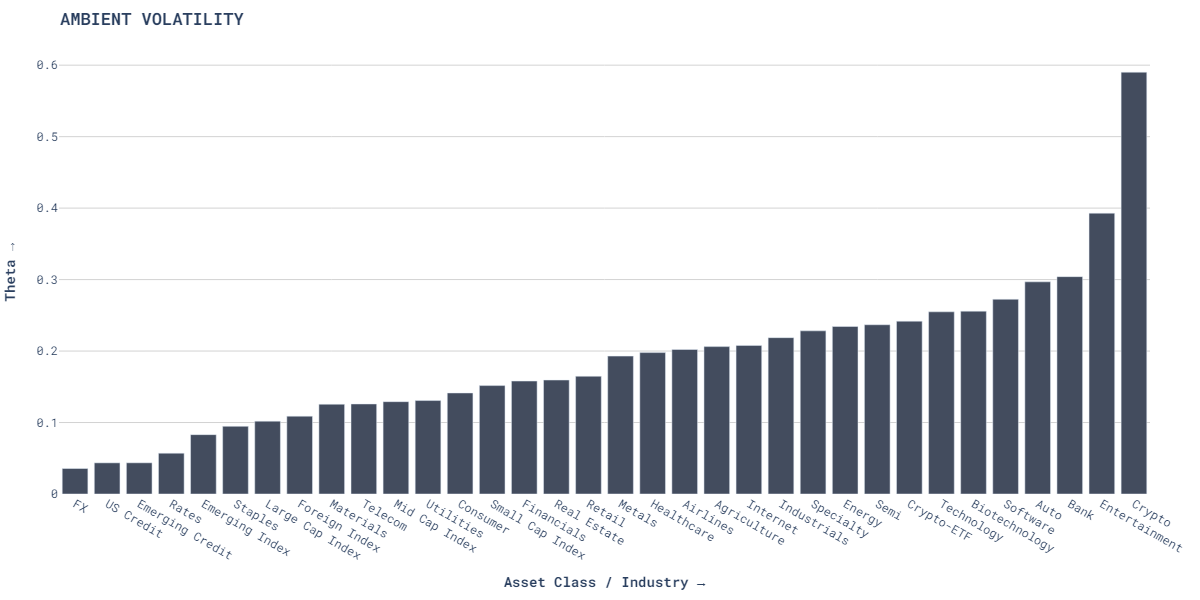
\includegraphics[width=\textwidth]{images/ambient_volatility_by_category.png}
    \caption{Ambient Volatility by Category}
    \label{fig:theta_by_category}
\end{figure}


The Cryptocurrencies which are deeply speculative in nature has an extraordinarily high ambient volatility compared to other asset classes. The entertainment industry which is mainly driven by consumer cyclicality seconds cryptocurrency in terms of long run volatility.
The sectors which are driven by innovation cycles and competitions such as technology biotechnology and automotive have relatively moderate ambient volatilities. The assets such as FX, Corporate and Treasury bonds  which are driven by macroeconomic factors such as interest rates, credit risks have the lowest levels of ambient volatility because their volatility are actively managed by central banks.


\subsubsection{ Mean Reversion $(\kappa)$}
The most interesting aspect of this kind of analysis is looking at the strength of mean reversion across tickers and asset classes.  The following chart shows the mean reversion rates as estimated by Ornestein-Ulhenback process aggregated for each sector. Although this chart is not very interpretable, therefore, in the next paragraph we modify the this mean reversion coefficient so as to look at expected time taken to reach the ambient volatility $(\theta)$ starting from a certain level of volatility. This helps to introduce interpretability in the mean reversion coefficient.

\begin{figure}[H]
    \centering
    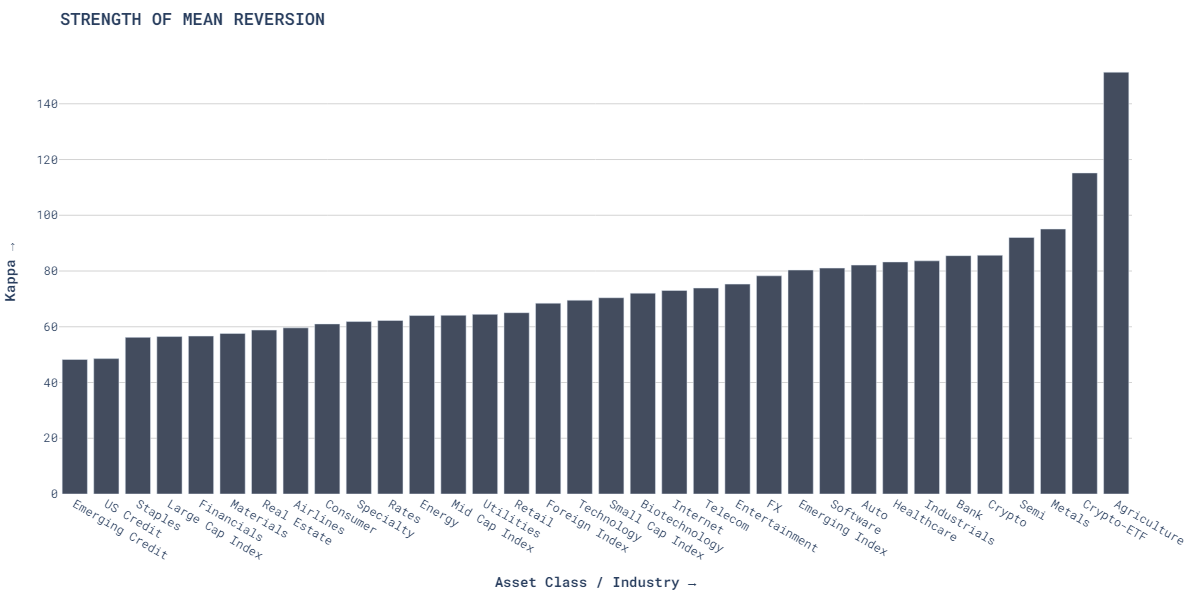
\includegraphics[width=\textwidth]{images/mean_reversion_by_category.png}
    \caption{Mean Reversion By Category}
    \label{fig:figure_label}
\end{figure}

Now since we know the mean reversion coefficient, we can ask another interesting question what is the expected amount of time it would take to reach from one level of volatility to another level of volatility. Since we have calibrated all the parameters of the stochastic differential equation, we can simulate different paths the volatility process could take which will enable us to look at the distribution of these Monte Carlo paths to estimate the parameter of interest.

To determine the expected amount of time that would elapse before the volatility touches its long run mean ($\theta$), we would first need to define, the first hitting or crossover time of the volatility process. Suppose we start from a volatility level $C$ and want to reach a volatility level of $A$. The expected time $T_{AC}$ can be expressed as an infimum over the set of all days $t$ where a single path crosses that volatility threshold.

$$ T_{A,C} = \inf\biggl\{ t\geq 0 \;: \; X_t = A \bigg| X_0 = C   \biggr\} $$

We can generate a large number of paths and the average of the infimums will give us the expected time to reach the level of ambient volatility.

To illustrate this concept, we can look at the iShares 20+ Year Treasury Bond ETF (TLT) which has a relatively slower mean reversion ($\kappa$) and we set the initial volatility level to be very high at 0.5, for the sake of a nice visualization. The estimated ambient volatility ($\theta$) of this ticker through Ornestien-Uhlenbeck process is 0.08. We generate 5000 Monte Carlo paths and we can observe that the volatility process is mean reverting to its ambient level over all the paths. To estimate the expected time to reach the ambient level, we take the average of the first crossovers over 5000 paths, which comes out to be 13.1 trading days with a standard error of 0.07 trading days.

\begin{figure}[H]
    \centering
    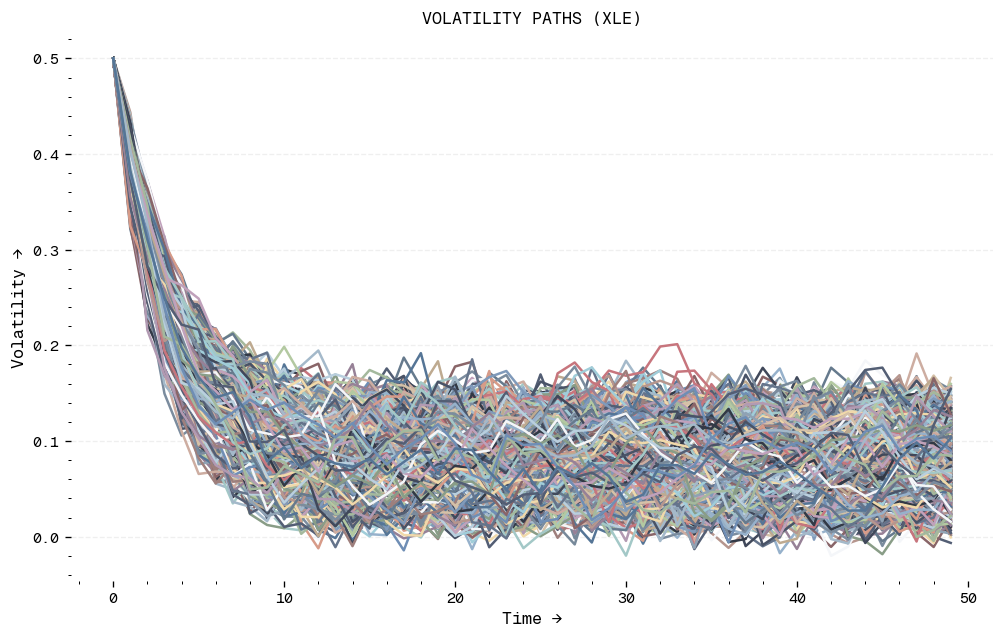
\includegraphics[width=\textwidth]{images/volatility_paths.png}
    \caption{Simulated 5000 paths of volatility process for TLT}
    \label{fig:figure_label}
\end{figure}

Please also note that very few volatility paths drop below zero. This is a Weiner process artefact and can be ignored, since we are looking at sufficiently large number of realizations.

A more interpretable version of looking at the mean reversion is to look at the expected number of days it will take for the volatility to reach its ambient level, given a starting level of volatility. The following chart shows the expected number of days it will take for the volatility to reach its ambient level ($\theta$) estimated through Ornestien-Uhlenbeck process for each industry / asset class, when we start from a pathologically high level of volatility of 0.5.

\begin{figure}[H]
    \centering
    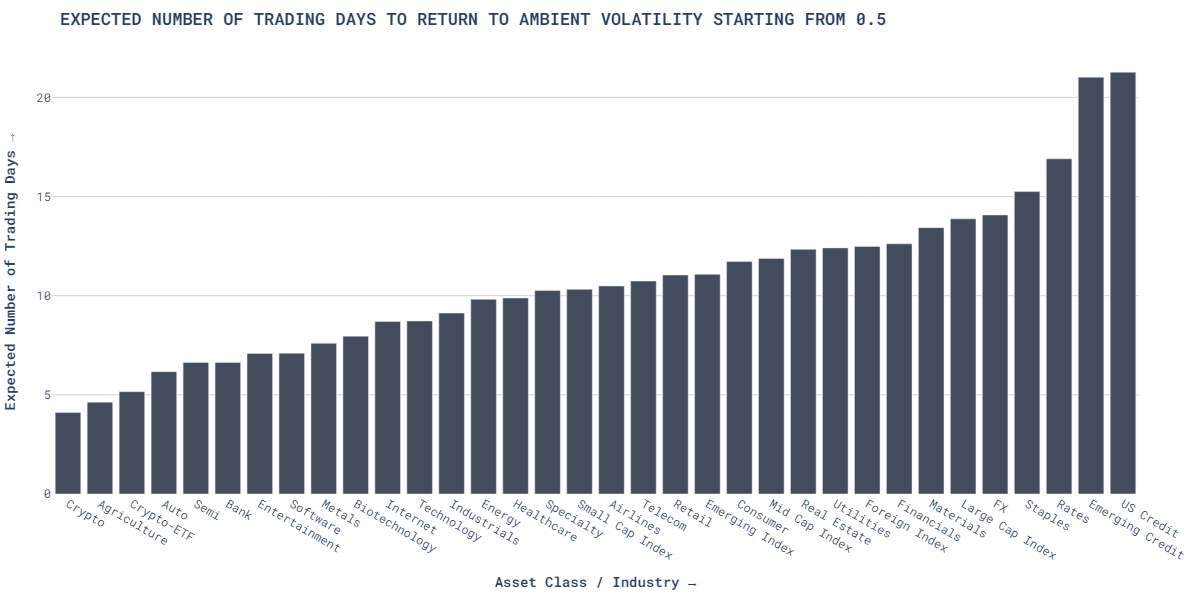
\includegraphics[width=\textwidth]{images/time_to_theta.png}
    \caption{Expected Time to Reach Ambient Volatility starting from a high volatility of 0.5}
    \label{fig:figure_label}
\end{figure}


If we start from a high volatility of 0.5, they take approximately four trading days to mean revert to their ambient volatility. A strong mean reversion tendency in agricultural tickers  is possibly due to the strong seasonal fluctuations inherent in these industries (\cite{Sorensen1999}). Cryptocurrency markets might be characterized by strong bursts of volatility which quickly stabilizes.

On the right end of the distribution, we have the industries that are highly sensitive to macroeconomic factors that influence credit markets such as Corporate bonds ETFs (HYG and LQD), Treasury Bond ETFs (TLT and IEF) of US and other emerging markets (EMB). These asset classes are heavily influenced by interest rates and default risks. Interest rate cycles usually span over several months and hence the volatility is expected to be persistent in these asset classes.

All the asset classes that relate to commodities and industrials like metal and energy sectors show reversion time around 6 to 8 trading days (starting from a high volatility) which indicates a relatively moderately persistent volatility.  The chart does not show the standard errors associated with each estimate of expected number of days however the standard error is extremely low possible because of a large sample realizations (5000 paths). The maximum standard error observed for the expected number of days over all tickers is one tenth of a trading day. The expected time levels as well as their associated standard errors for each ticker is shown in the appendix.

One more interesting insight emerges when we look at the scatter of the mean reversion against ambient volatility. 

\begin{figure}[H]
    \centering
    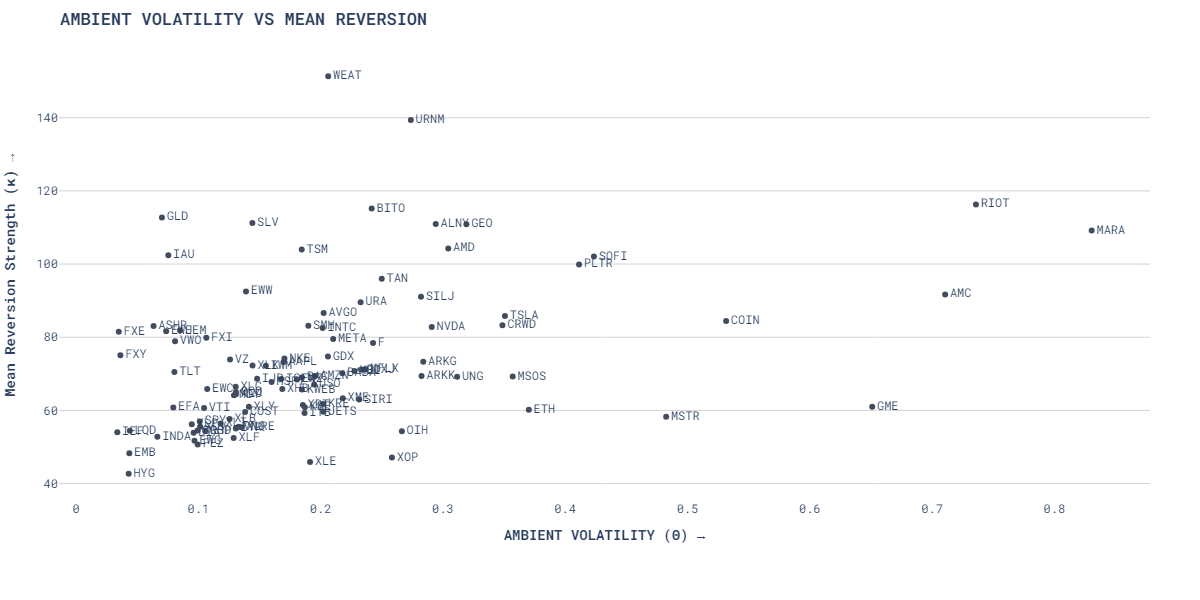
\includegraphics[width=\textwidth]{images/ambient_volatility_vs_mean_reversion.png}
    \caption{Scatter of Ambient Volatility vs Mean Reversion}
    \label{fig:figure_label}
\end{figure}

The strength of mean reversion has a heteroscedastic relationship with ambient volatility that is the variability of mean reversion across the cross section of tickers is conditional on what level of ambient volatility we are looking at.  At the lower levels of ambient volatility we find a strong visible correlation between the strength of mean reversion and ambient volatility which further dampens as we move to higher levels of ambient volatility across the cross section of tickers.



\subsubsection{ Meta Volatility $(\sigma)$  }

The meta volatility is the volatility of the volatility. The following chart shows the meta volatility as estimated by Ornestein-Ulhenback process aggregated for each industry / asset class.

\begin{figure}[H]
    \centering
    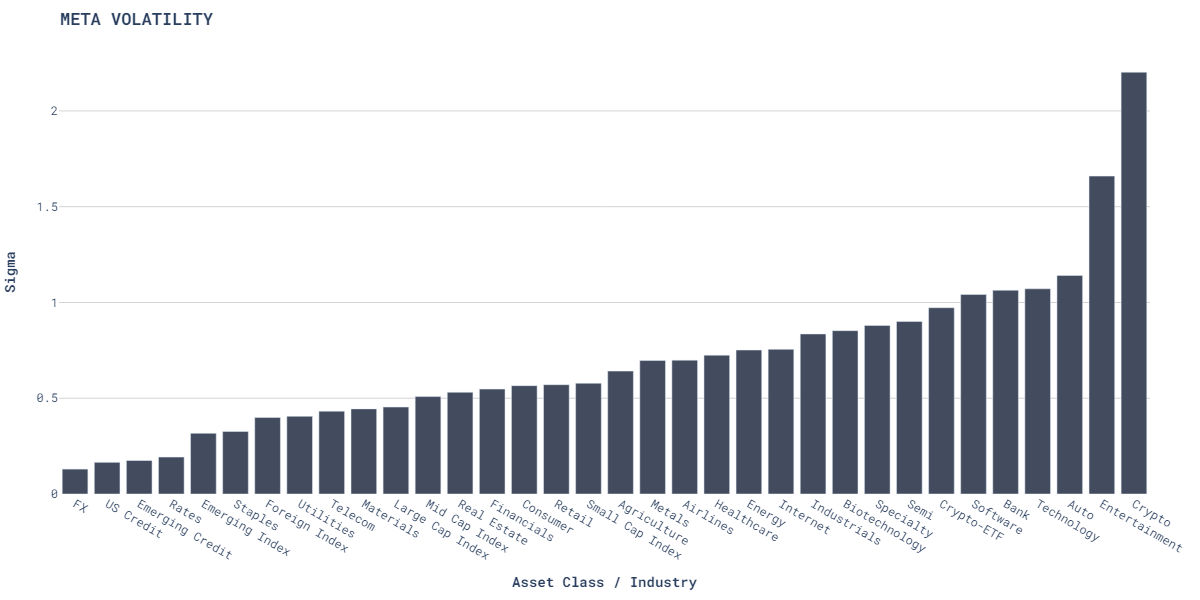
\includegraphics[width=\textwidth]{images/meta_volatility_by_category.png}
    \caption{Meta Volatility by Asset Class}
    \label{fig:figure_label}
\end{figure}

A truly interesting insight here is that this chart looks very similar to the ambient volatility chart in Figure \ref{fig:theta_by_category}. The empirical implication here is that if a asset class is characterized by a high level of ambient volatility, the volatility inherent in the ambient volatility is also high. This is apparently visible if we  look at the scatter of meta volatility against the ambient volatility.

\begin{figure}[H]
    \centering
    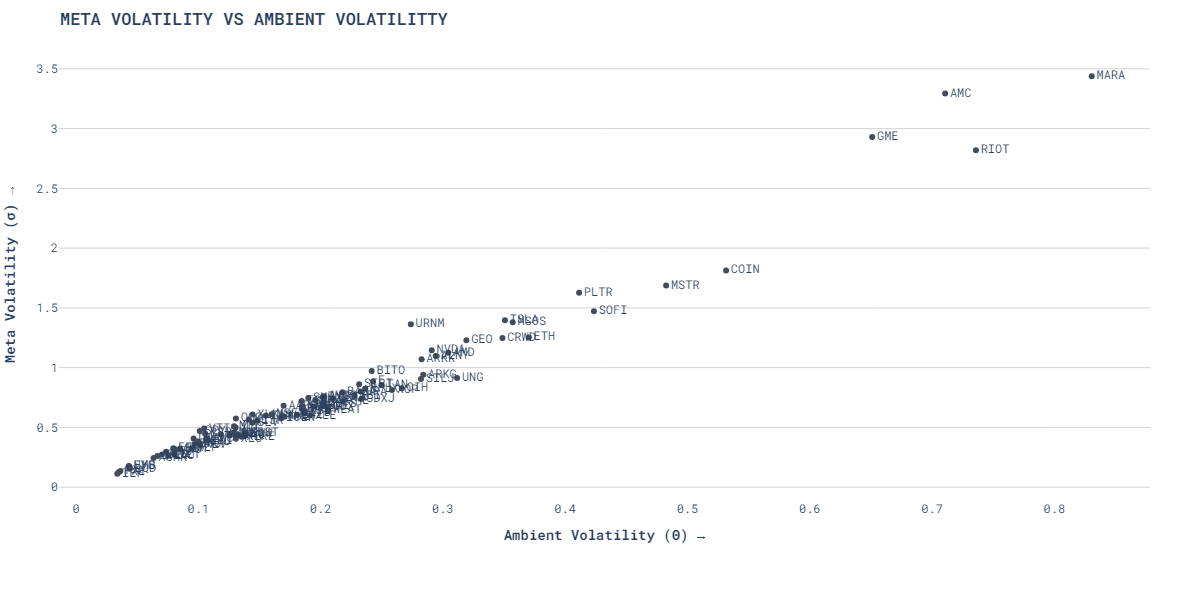
\includegraphics[width=\textwidth]{images/meta_volatility_vs_ambient_volatility.png}
    \caption{Scatter of Meta Volatility vs Ambient Volatility}
    \label{fig:figure_label}
\end{figure}

The relationship of meta volatility with the strength of mean reversion is similar to the relationship of ambient volatility with that of mean reversion. This is evident in the scatter below.

\begin{figure}[H]
    \centering
    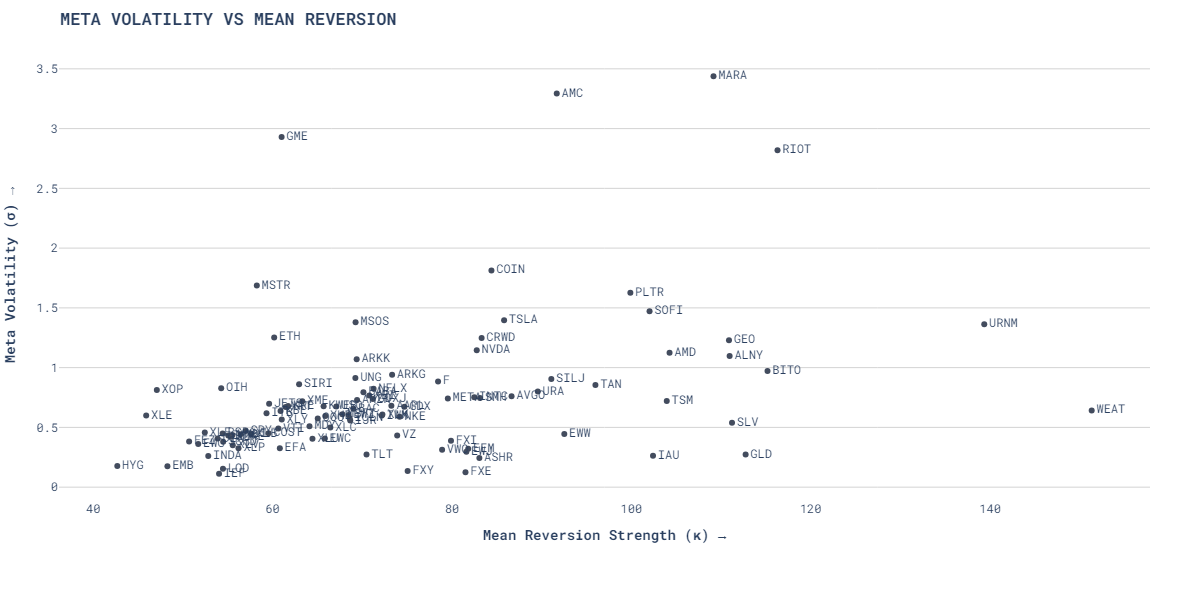
\includegraphics[width=\textwidth]{images/meta_volatility_vs_mean_reversion.png}
    \caption{Scatter of Meta Volatility vs Mean Reversion}
    \label{fig:figure_label}
\end{figure}

\section{ Roadmap from here}

\begin{displayquote}

“Forty-two!" yelled Loonquawl. "Is that all you've got to show for seven and a half million years' work?"  "I checked it very thoroughly," said the computer, "and that quite definitely is the answer. I think the problem, to be quite honest with you, is that you've never actually known what the question is.”  - Douglas Adams, The Hitchhiker’s Guide to the Galaxy

\end{displayquote}

Now I will venture into options market from the underlying spot markets.  The options market gives me two additional pieces of information that is the implied volatility and the skew.  At this point, I have a powerful model for the realised volatility.  This will enable me to ask good questions about  the implied volatility and the markup of the implied and the realised volatility that is the volatility risk premium.

\begin{enumerate}
\item Every trading day I can measure the distance between the realised volatility from the ambient volatility. The farther is the the realised volatility from the ambient volatility, it will be interesting to see how Volatility Risk Premium moves. Using these insights, can I find options that are mispriced or priced cheaply in the market?
\item I can use the gap between realised volatility and ambient volatility to see if market is overreacting to short term volatility bursts. This could be an incredibly useful trading signal.
\item Is the current implied volatility accurately pricing the future realized volatility? Is there a pattern when implied volatility consistently overshoots or underpredicts the future realised volatility.
\item I also know the mean reversion speed of the volatility process for each ticker. This can reveal potential mispricing of short term options.
\item How does the skew move with realized volatility?
\item How is skew distributed across asset classes?
\end{enumerate}


These questions would change and evolve as I move forward in the thesis. I am not sure, if I am still asking the right questions. The questions would themselves appear with the data. Motion creates information. Peace.



\section[Option Markets]{Options and Volatility}
\subsection{Option price is about Volatility}

In this section, I will motivate that, in the absence of any directional bias- meaning that one does not care if the underlying price rises or falls, the price of an option is only dependent upon the volatility and the time to expiration. This can be mathematically shown by deriving the price of a straddle starting with Black Scholes option pricing formula.  
The Black-Scholes formula spot price $S_0$ and the strike price $K$ is given as:

$$
C = S_0 \Phi(d_1) - K e^{-r T} \Phi(d_2)
$$

Where $d_1$ and $d_2$ are defined as:

$$
d_1 = \frac{\ln\left(\frac{S_0}{K}\right) + \left(r + \frac{\sigma^2}{2}\right)T}{\sigma \sqrt{T}}
$$

$$
d_2 = d_1 - \sigma \sqrt{T}
$$

This represents the intrinsic value of the option that is how much in the money is the option, right now. For an ATM option, this term would be 0. Assuming a zero cost of carry (risk free rate plus the dividend yield), the pricing formula simplifies to:

Assuming the risk-free rate \( r = 0 \), the expressions simplify as follows:

$$C = S_0 \left( \Phi(\frac{\sigma \sqrt{T}}{2}) - \Phi(-\frac{\sigma \sqrt{T}}{2}) \right)$$

Similarly, for a put option $P$, this formula is:

$$ P = S_0 \left( \Phi(-\frac{\sigma \sqrt{T}}{2}) - \Phi( \frac{\sigma \sqrt{T}}{2}) \right) $$

Now we will price an ATM straddle which involves buying both a call and a put option, the price $C + P$ can be written as:

$$C + P = S_0 \left( \Phi(d_1) - \Phi(d_2) \right) + S_0 \left( \Phi(-d_2) - \Phi(-d_1) \right)$$

Using the symmetry of the normal distribution i.e.: $\Phi(-x) = 1 - \Phi(x)$

This simplifies to:

$$C + P = 2 S_0 \left( \Phi(d_1) - \Phi(d_2) \right)$$

$$C + P = 2 S_0 \left( \Phi\left( \frac{\sigma \sqrt{T}}{2} \right) - \Phi\left( -\frac{\sigma \sqrt{T}}{2} \right) \right)$$

Now again applying the notion of symmetry i.e. $\Phi\left( -\frac{\sigma \sqrt{T}}{2} \right) = 1 - \Phi\left( \frac{\sigma \sqrt{T}}{2} \right)$, the final expression becomes:

$$C + P = 2 S_0 \left( 2\Phi\left( \frac{\sigma \sqrt{T}}{2} \right) - 1 \right)$$

$\Phi$ is the CDF of standard normal distribution which is an increasing function. 

The expression for the straddle price is interesting for two reasons:
\begin{enumerate}
    \item We can infer from this expression given an expiration, the only thing that drives the value of an option is the volatility term $\sigma$. 
    \item Given a level of volatility, the value of straddle grows at the rate of square root of time.
\end{enumerate}

In the succeeding sections, we will be looking at the unconditional distributions of volatility and volatility risk premium across assets and deriving insights.

\section[Assumptions and Challenges]{Assumptions and Challenges}
\subsection{Assumptions on Implied Volatility}
Implied Volatility is a market view of future volatility. Market view can be influenced by a lot of systematic and idiosyncratic factors. Unlike other parameters like the current spot price, strike price, cost of carry and the time to expiration which can be directly observed, the volatility is not directly measurable because of its forward looking nature. The \cite{RateLab2008} remarks implied volatility as a measure of fear. Here the authors use the Merrill Lynch move index which measures the implied volatility in US Treasury options to signify how low levels of implied volatility often precedes sharp increases in volatility. Furthermore, implied volatility is influenced by the term structure. As options get closer to maturity, the expectation around implied volatility changes significantly as the uncertainty reduces. The focus of this analysis is on the short term options. The expiration of the options range from 31 days to 1 day. 
One thing that I need to confess upfront that I have completely ignored the term structure of implied volatility since I am working with short-term options that is the days left to expiry range from 1 to 31 days. This assumption can be defended on two grounds:
1. The short-term options have a low vega. That is, their price is not very sensitive to changes in implied volatility.    
2. Although the vega risk is low, the volatility of implied volatility is higher for short-term options. This means that you do not have a systematic shape of term structure of volatility when you are looking at options that are going to expire in few days.    
One of the key characteristics of volatility is that if you look at the volatility time series, the time series is usually stationary. This is a nice feature to have because this allows us to look directly at the distributions across different tickers and compare them. The volatility distribution also has very long and fat tail because of the clustering and sharp spikes. 


\subsection{Assumptions on Realised Volatility}
In order to construct the volatility risk premium for an option contract, we need to have an estimate of realised volatility. Has also explained in the preceding sections this can be done in several ways and hence it is not a trivial problem to solve. In this paper the estimate for the realised volatility would be the simple annualized standard deviation sampled at 5 minute intervals over a lookback period equal to the time left for expiration. 
Suppose an option contract is priced on 3rd February 2020 at 9:35 AM with an expiration on 21st February 2020. There are 18 days left for expiration. Hence the lookback period for the realized volatility would be from 07th January 2020 9:35 AM shifted back by 18 days that is 3rd February 2020 9:35 AM. We will calculate the simple standard deviation of five minute log returns in this lookback period and will annualize it. Also note that the US holidays and weekends are also taken into consideration while calculating the lookback horizon. Therefore, for every option contract that is priced in the market the realized volatility estimate is dynamically calculated by looking at the time that is left for expiration. This makes the realised volatility more representative of the specific time horizon relevant to the lifetime of the option which adds robustness to the analysis.

$$ RV= \sqrt{252 \times 6.5 \times 12} \times \sqrt{\frac{1}{N_{5m}-1} \sum_{i=1}^{N_{5m}} (r_i - \bar{r})^2} $$  

Here $N_{5m}$ is the number of 5 minute intervals in the lookback period.

\subsection{Moneyness or Delta?}
Another important insight to note here is that delta represents hedge ratio and not a probability. This assumption is especially crucial  Delta is usually interpreted as the probability of an option finishing in the money. However this is only true if the return distribution is balanced, which means the volatility is low.  When the price process of the underlying is volatile, such as cryptocurrency or biotechnology stocks, more delta will diverge from the probability (\cite{abdelmessih2020lessons}).  Intuitively, a 10\% out of the money option for a cryptocurrency is more likely to finish in the money than a 10\% out of the money option for a utility or retail stock. During the course of this paper, we will treat 50-Delta options as a standard for comparison across tickers. 


\subsection{Cost of Hedging}
Another important insight to note here is that the implied volatility also accounts for the hedging cost that the market maker uses to price the option. The market maker does not have any directional bias and it is apparent from the mathematical derivation using the Black Scholes formula that is also shown above that any cost above the intrinsic value of the option would reflect in the implied volatility. Furthermore the cost of hedging is directly dependent on the volatility and therefore it is incredibly difficult to distil implied volatility into pure volatility risk premium and the cost of hedging. The focus of this paper would be to look at the distributions of the volatility risk premium and skew and derive exploratory insights.

\subsection{Selection of Tickers}

We will laser this analysis on the call options for the following underlying tickers and asset classes. 
\begin{table}[h]
    \centering
    \begin{tabular}{|c|c|c|}
        \hline
        \textbf{Ticker} & \textbf{Category} & \textbf{Trade Name} \\
        \hline
        FXY & FX & CurrencyShares Japanese Yen Trust \\
        FXE & FX & CurrencyShares Euro Trust \\
        GLD & Shiny Metals & SPDR Gold Shares \\
        SLV & Shiny Metals & iShares Silver Trust \\
        TLT & Rates & iShares 20+ Year Treasury Bond ETF \\
        IEF & Rates & iShares 7-10 Year Treasury Bond ETF \\
        HYG & US Credit & iShares iBoxx \$ High Yield Corporate Bond ETF \\
        LQD & US Credit & iShares iBoxx \$ Investment Grade Corporate Bond ETF \\
        EMB & Emerging Credit & iShares J.P. Morgan USD Emerging Markets Bond ETF \\
        VWO & Emerging Index & Vanguard FTSE Emerging Markets ETF \\
        IJR & Small Cap Index & iShares Core S\&P Small-Cap ETF \\
        IWM & Small Cap Index & iShares Russell 2000 ETF \\
        MDY & Mid Cap Index & SPDR S\&P MidCap 400 ETF Trust \\
        SPY & Large Cap Index & SPDR S\&P 500 ETF Trust \\
        XLE & Energy & Select Sector SPDR Fund - Energy \\
        AMD & Semi & Advanced Micro Devices, Inc. \\
        TSM & Semi & Taiwan Semiconductor Manufacturing Company Limited \\
        INTC & Semi & Intel Corporation \\
        NVDA & Semi & NVIDIA Corporation \\
        TSLA & Auto & Tesla, Inc. \\
        F   & Auto & Ford Motor Company \\
        \hline
    \end{tabular}
    \caption{Ticker Symbols, Categories, and Trade Names}
    \label{tab:ticker_symbols}
\end{table}

These asset classes would be color coded as follows:

\begin{figure}[H]
    \centering
    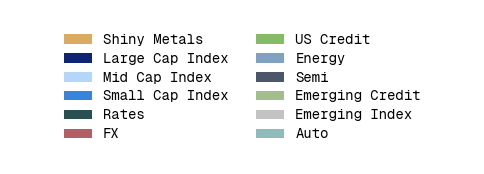
\includegraphics[width=0.8\textwidth]{images/ticker_color_code.png}
    \caption{Color coding for different asset classes}
    \label{fig:asset_class_colors}
\end{figure}


\section[The Implied and the Realised Volatility]{Relationships between Implied and the Realised Volatility}
\subsection{Correlations and Clustering between the Implied and the Realised Volatility}
A simple scatter plot of the implied volatility and the realised volatility reveals interesting very insights. Note that sample is limited to 50-Delta options.

\begin{figure}[H]
    \centering
    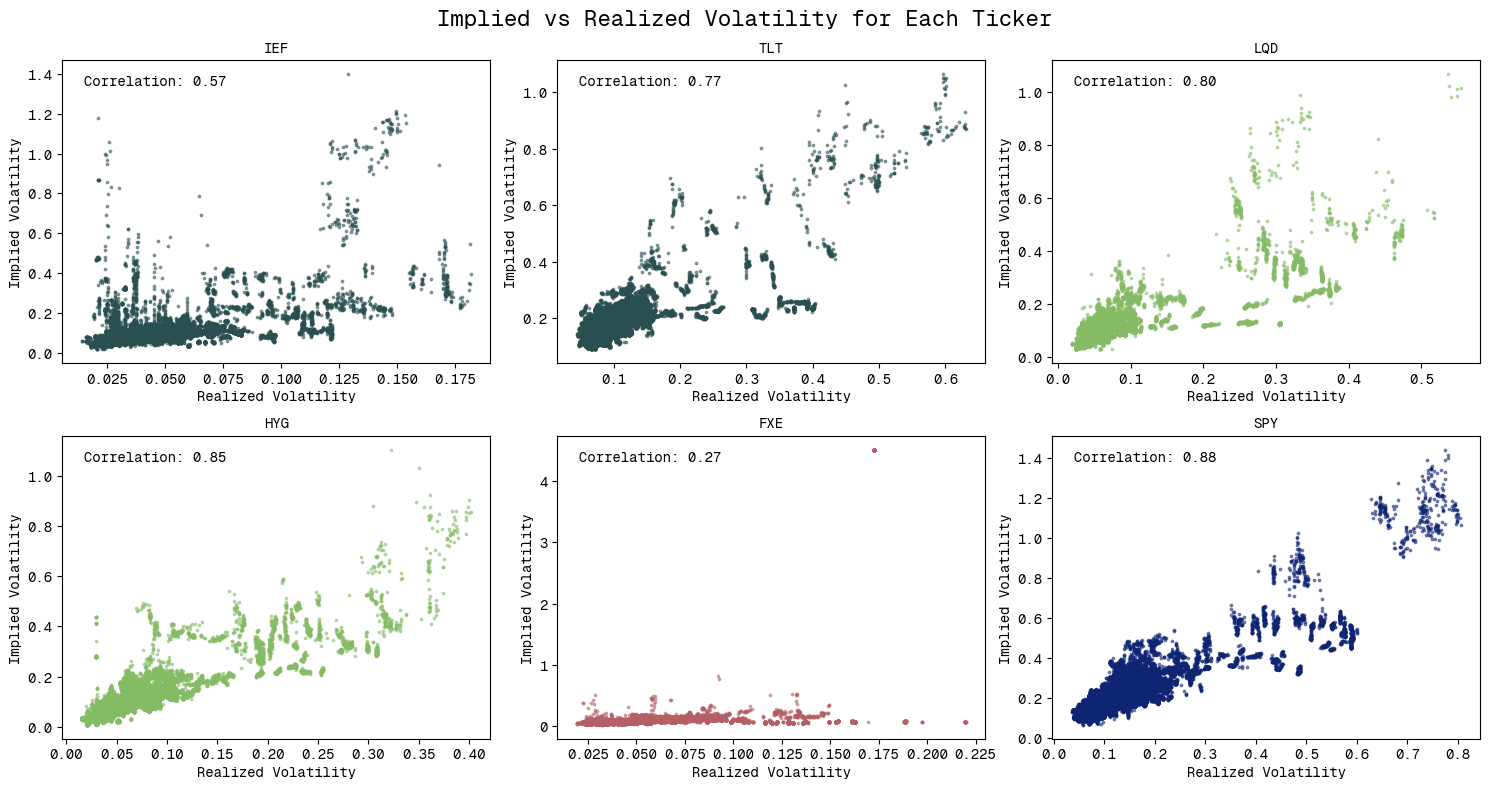
\includegraphics[width=1\textwidth]{images/iv_and_rv_batch1.png}
    \caption{Implied and the Realised Volatility}
    \label{fig:iv_and_rv1}
\end{figure}

We find a very high correlation between implied volatility (IV) and realized volatility (RV) for iShares 20+ Year Treasury Bond ETF (TLT), iShares iBoxx \$ Investment Grade Corporate Bond ETF (LQD), SPDR S\&P 500 ETF Trust (SPY), and iShares iBoxx \$ High Yield Corporate Bond ETF (HYG). However, CurrencyShares Euro Trust (FXE) stands out. Contrary to other tickers, it is the only one that exhibits extremely low correlation. Another interesting phenomenon is the clustering of points at the north-east corner of SPDR S\&P 500 ETF Trust (SPY) ticker. It appears as if the implied volatility tends to overshoot once a certain threshold of realized volatility has been crossed for this ticker. What explains this phenomenon could be an interesting research question and a hot-bed for a machine learning predictive model. A similar clustering is also observed for the small-cap index - iShares Russell 2000 ETF (IWM) and shiny metals (GLD and SLV).

\begin{figure}[H]
    \centering
    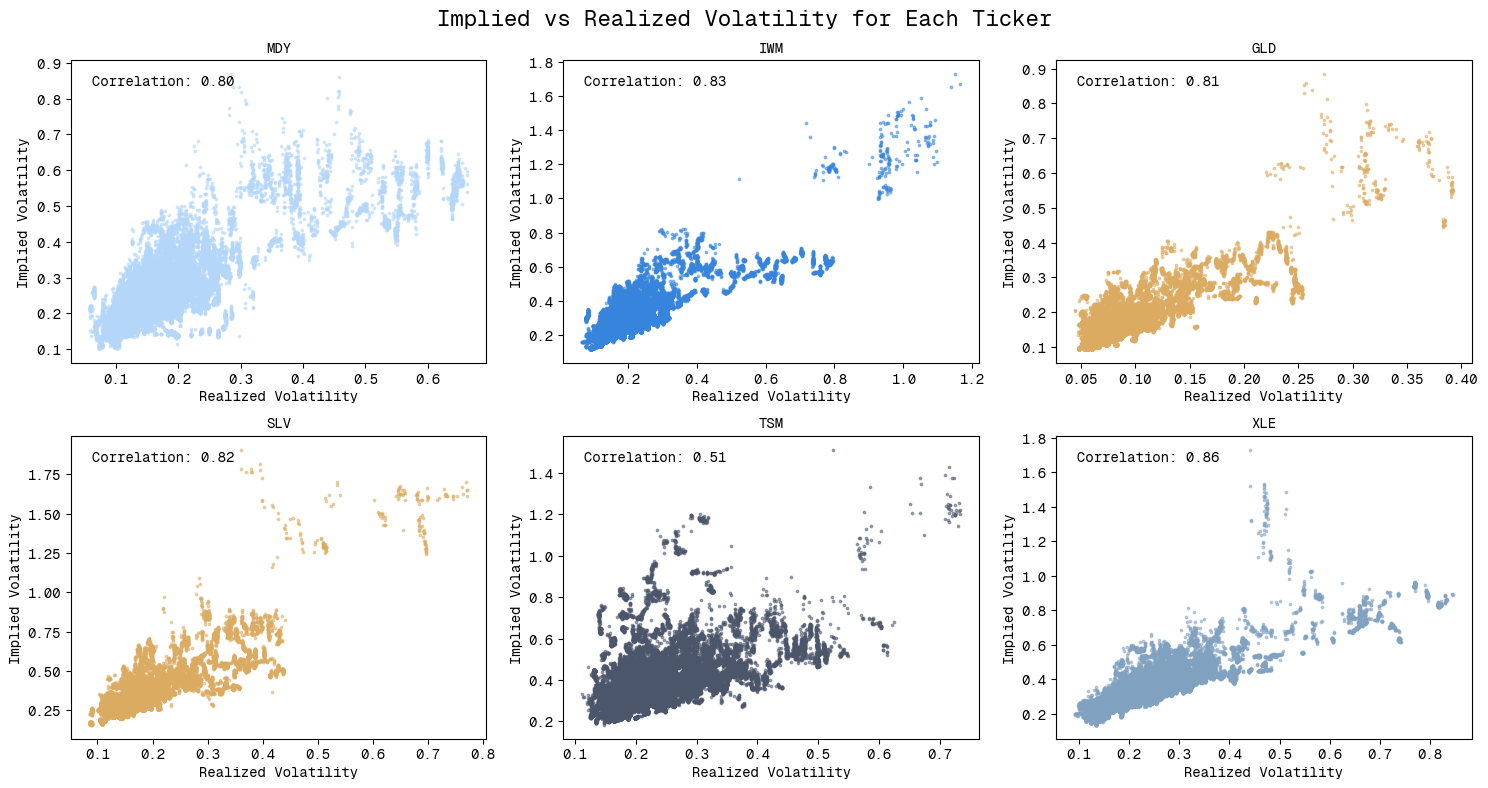
\includegraphics[width=1\textwidth]{images/iv_and_rv_batch2.png}
    \caption{Implied and the Realised Volatility}
    \label{fig:iv_and_rv2}
\end{figure}

The insights turn even more interesting when we look at OTM call options that is the contracts with deltas between 0.2 and 0.3. The high correlation vanishes for almost every ticker. However, what is common is a cone like shape for almost every ticker. The interpretation is that when the realised volatility is low the implied volatilities are clustered at the lower end in a narrow area. As the uncertainty increases, the range of implied volatilities that are observed becomes wider. 

\begin{figure}[H]
    \centering
    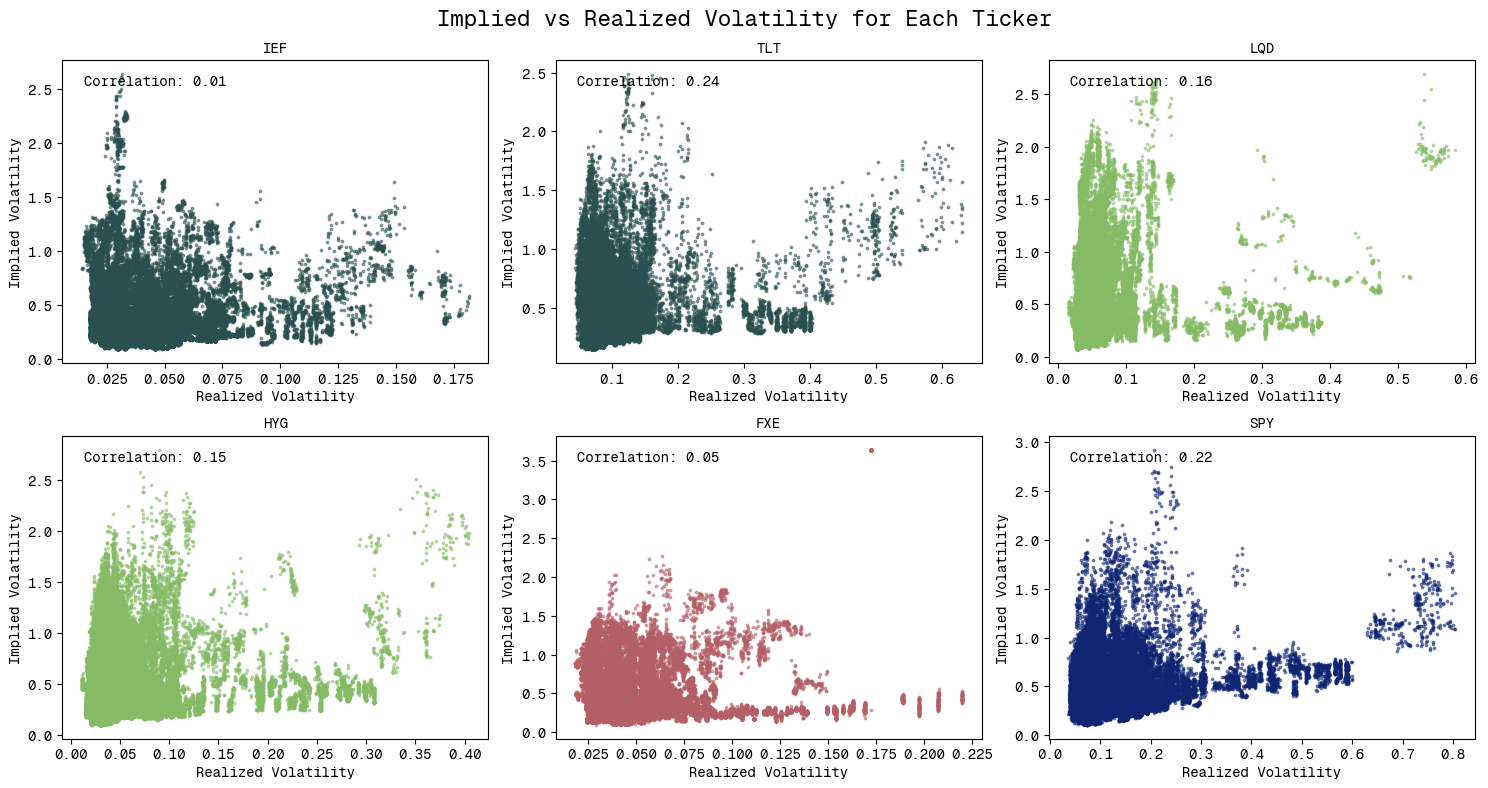
\includegraphics[width=1\textwidth]{images/iv_and_rv_otm_batch1.png}
    \caption{Implied and the Realised Volatility}
    \label{fig:iv_and_rv__otm_1}
\end{figure}

\begin{figure}[H]
    \centering
    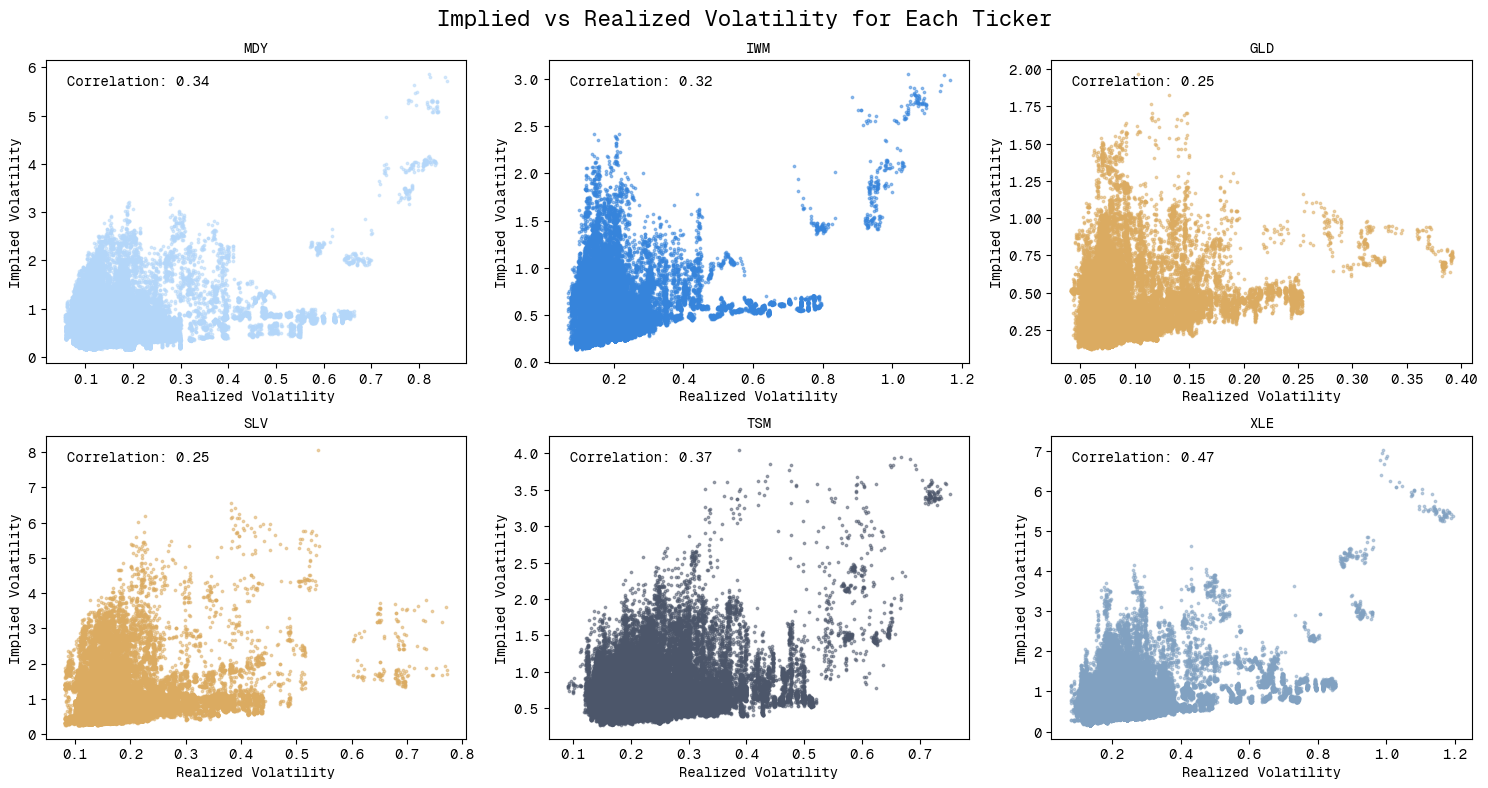
\includegraphics[width=1\textwidth]{images/iv_and_rv_otm_batch2.png}
    \caption{Implied and the Realised Volatility}
    \label{fig:iv_and_rv__otm_2}
\end{figure}

Now having looked at the joint distributions of IV and RC, we will move on to the volatility risk premium.

\section[VRP]{Volatility Risk Premium}
\subsection{VRP of 50-Delta Options}

The volatility risk premium is expressed as a simple ratio of the implied volatility priced into the options contract and the realized volatility computed from the methodology mentioned above. 
$$ VRP = IV / RV $$
The following violin plot shows the distribution of the volatility of the volatility risk premium across different tickers and asset classes.

\begin{figure}[H]
    \centering
    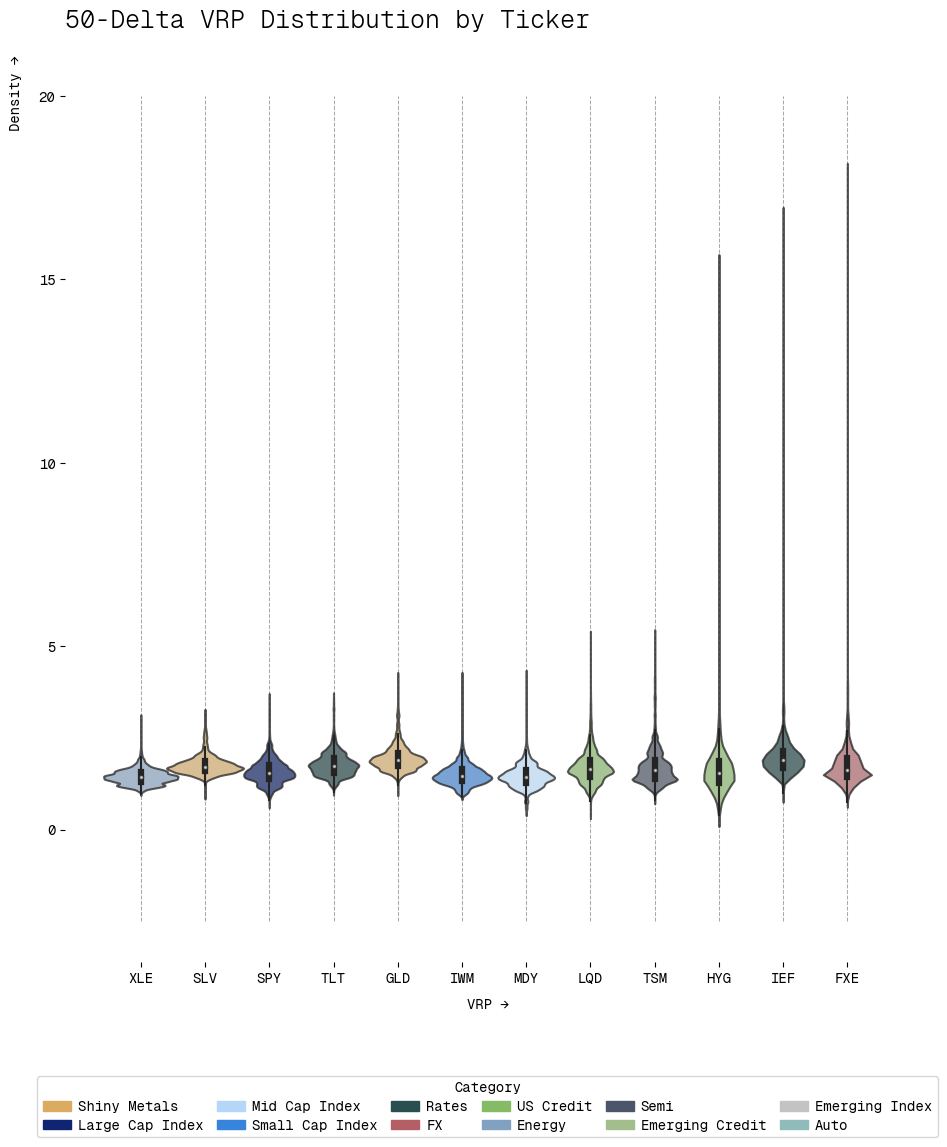
\includegraphics[width=1\textwidth]{images/atm_vrp_violin.png}
    \caption{Distribution of Volatility Risk Premium}
    \label{fig:atm_vrp_violin}
\end{figure}


There are few interesting and apparent insights:
\begin{enumerate}
    \item The ticker which have visibly very long tails are the tickers that are directly affected by interest rates, for example, currency values,  Treasury bond ETFs and credit ETFs.  In the preceding section where we modelled the realized volatility, we have already shown that the interest rate dependent tickers show the slowest mean reversion or a high persistence of volatility. This makes intuitive sense because a lingering volatility would also keep the volatility risk premium high as mean reversion is slow. This could also very well be a data artefact. The last five years which is also the time period of the sample, have seen many interest rate regimes and the market has been pricing in a lot of uncertainty.  These long tails in interest rate dependent tickers appear likely to happen around FOMC meetings. It is interesting to note that the the 20 year treasury bond ETF (TLT) is an exception to this phenomenon probably due to its long term nature.
    \item The volatility risk premium also show a richer variation among different asset classes. This is apparent when we look at the univariate distributions for few tickers. Here, the Gold commands the highest volatility risk premium as the distribution looks significantly to the right that is followed by 20 year Treasury bonds. The VRP of the Energy ETF (XLE) has the lowest variability while the VRP of the Large Cap Index (SPY) has the highest variability. 
\end{enumerate}

\begin{figure}[H]
    \centering
    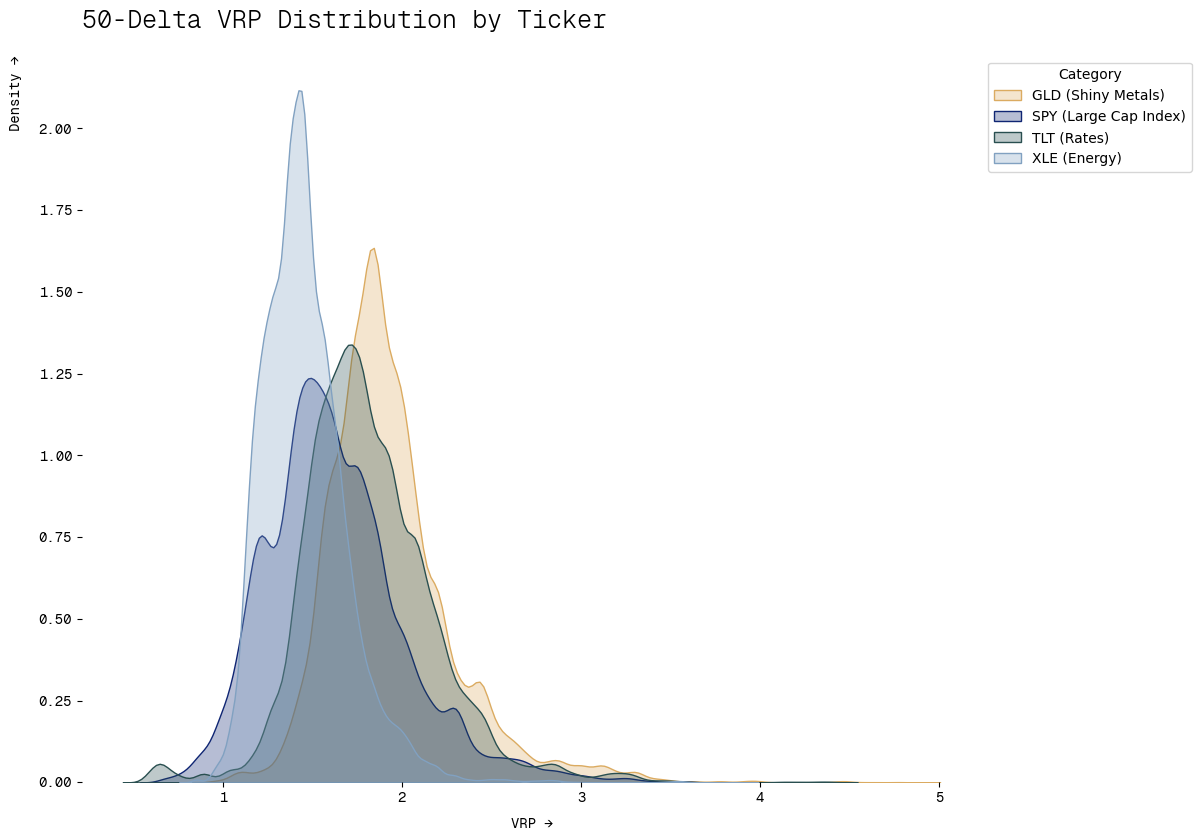
\includegraphics[width=1\textwidth]{images/kde_vrp_atm.png}
    \caption{Distribution of Volatility Risk Premium}
    \label{fig:kde_vrp_violin}
\end{figure}


When we look at the VRP of the OTM options, they are dominated by extremely heavy tails, the length of tails again look highly correlated with interest-rate dependence.

\subsection{VRP of 25 to 30-Delta Options}

When we look at the VRP of the OTM options, they are dominated by extremely heavy tails, the length of tails again look highly correlated with interest-rate dependence.

\begin{figure}[H]
    \centering
    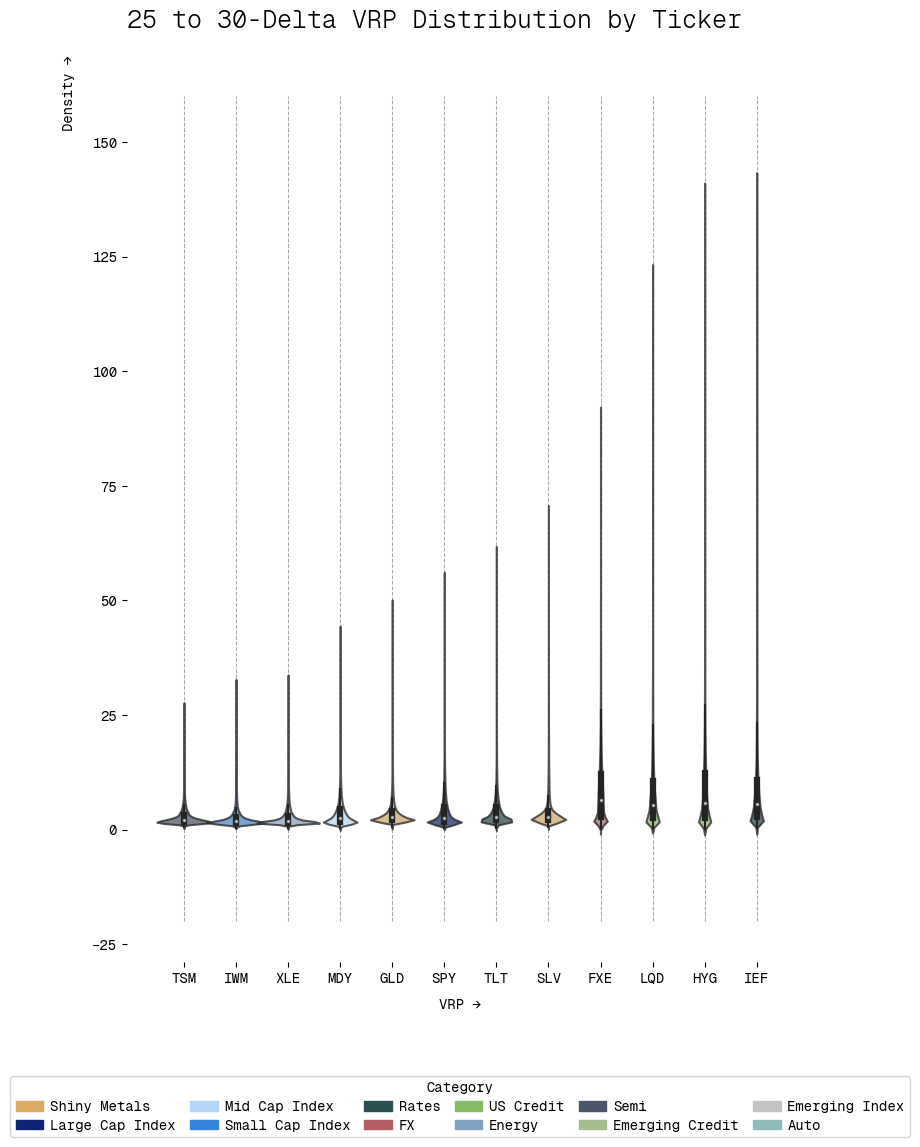
\includegraphics[width=1\textwidth]{images/otm_vrp_violin.png}
    \caption{Distribution of Volatility Risk Premium}
    \label{fig:otm_vrp_violin}
\end{figure}

\section[Skew]{Skew}
\subsection{What is skew and what does it measure? }

\cite{das1998smiles} have eloquently answered this question in the introduction of the paper. As per the theoretical framework of Black and Scholes, the implied volatility is independent of the strike price for a given expiration, since the implied volatility is an input parameter to the model used to price the option. As per \cite{das1998smiles}, the volatility smile stems from the presence of excess kurtosis in the conditional returns distribution and an asymmetry in the volatility smile is due to the skewness in this distribution.

Another study by \cite{mixon2011volatility} provides an extensive literature review for different measures of skew in options markets. The paper identifies that the ad hoc measures of skewness lack a rigorous justification because they do not control for volatility and kurtosis implicit in the distribution. The author presents the normalised difference between a 25-Delta put and a 25-Delta call which he argues to be the least redundant among the other competitor metrics that he analysed. The measure of skewness that we have used in this paper is directly taken from \cite{mixon2011volatility}, which is:
$$ \text{Skew} = \frac{IV_\text{25D-Put} - IV_\text{25D-Call}}{IV_\text{50D-Put} } $$

However, for now, I will keep it very simple. The skew is calculated as the difference between the implied volatility of 25-Delta call and 50-Delta Call.
$$ \text{Skew} = \frac{IV_\text{25D-Call}} {IV_\text{50D-Call}}$$



\textit{Note to instructor, to be removed later: Right now I just wanted to see how the skew looks like. A proper measure of skew would require a bit more careful and involved work as I would need to join the call option contracts with their counterpart put options contracts.}


The distribution of skew looks very similar to the the distribution of the OTM implied volatility. It is characterized by very long tails and a high variability especially for the interest rate dependent tickers. 


\begin{figure}[H]
    \centering
    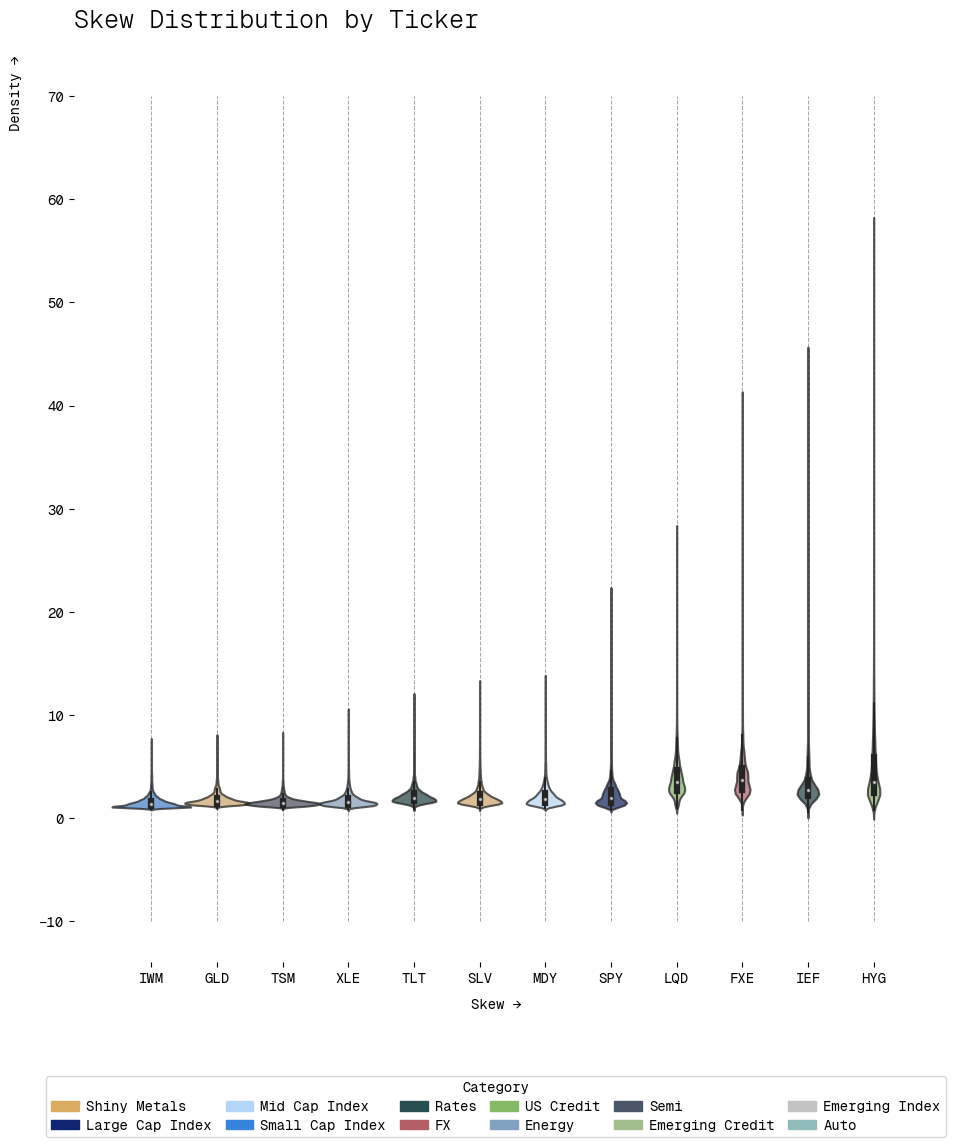
\includegraphics[width=1\textwidth]{images/skew_violin.png}
    \caption{Distribution of Skew}
    \label{fig:skew_violin}
\end{figure}

The relationship of skew is also similar to those of OTM IVs that is a cone like shape for almost every ticker. The interpretation is that when the realised volatility is low the skew clustered at the lower end in a narrow area. As the uncertainty increases, the range of skews that are observed becomes wide.

\begin{figure}[H]
    \centering
    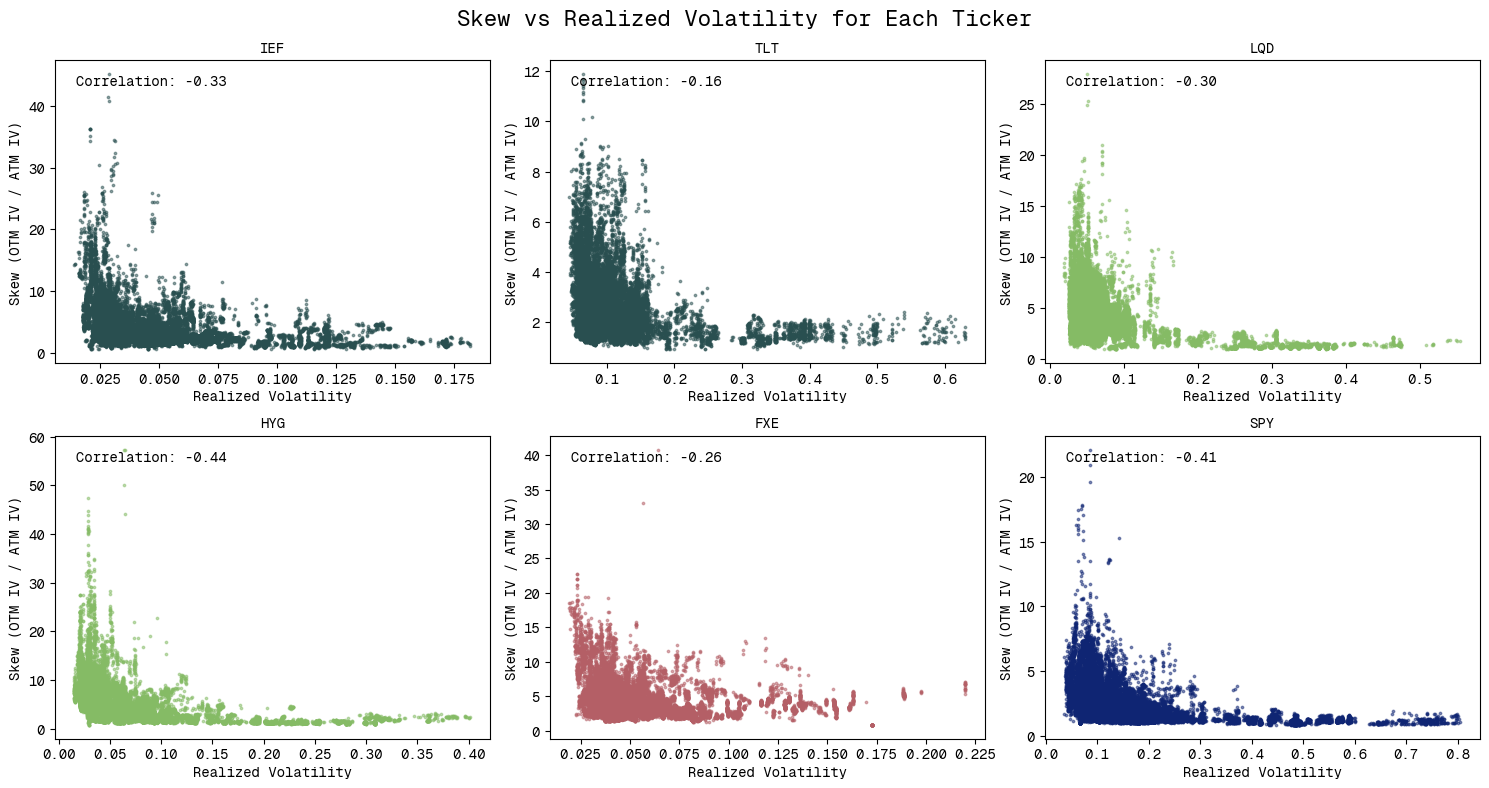
\includegraphics[width=1\textwidth]{images/skew_and_rv_otm_batch1.png}
    \caption{Distribution of Skew}
    \label{fig:skew_and_rv_otm_batch1}

    
\end{figure}
    \begin{figure}[H]
        \centering
        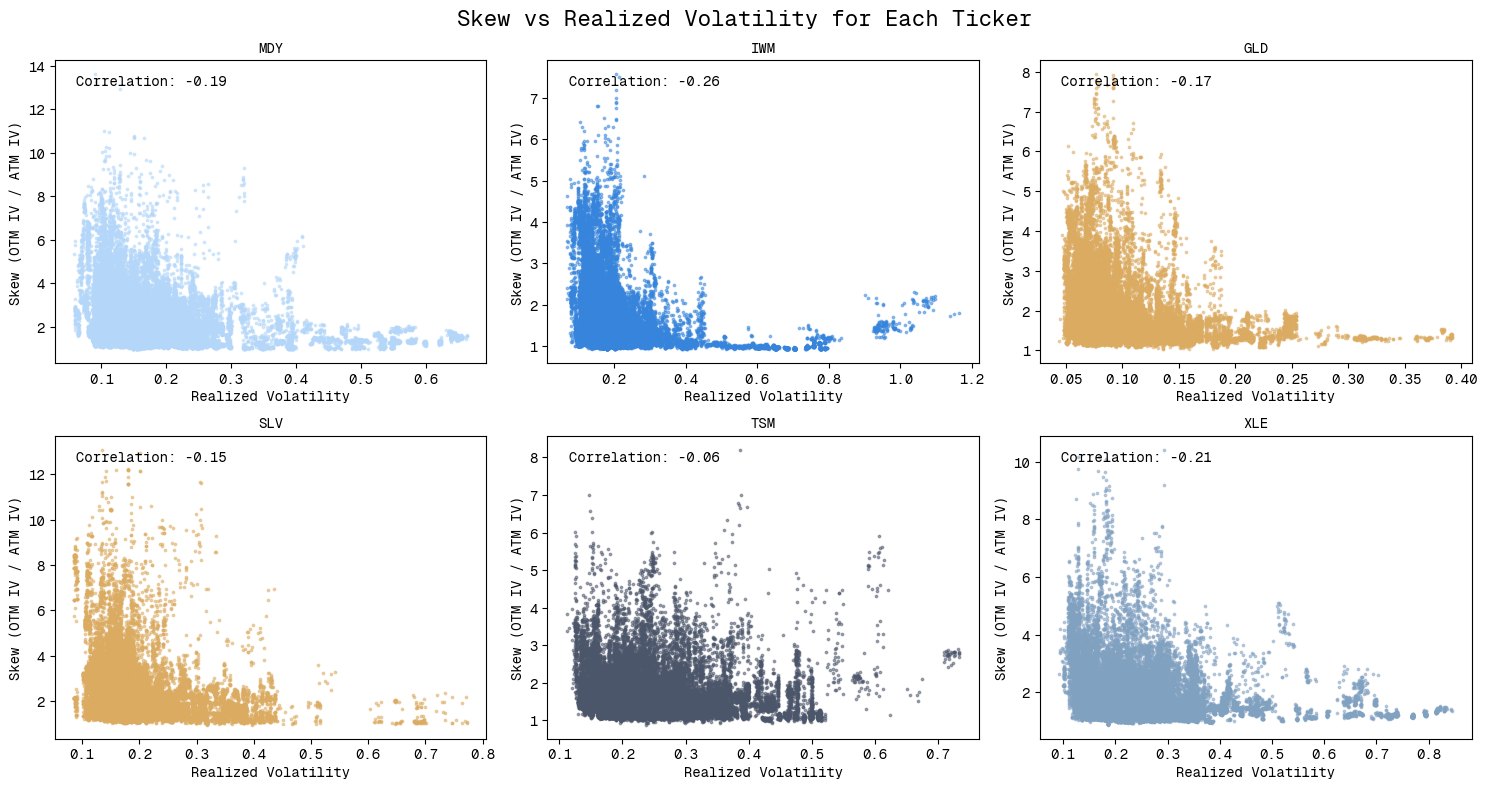
\includegraphics[width=1\textwidth]{images/skew_and_rv_otm_batch2.png}
        \caption{Distribution of Skew}
        \label{fig:skew_and_rv_otm_batch2}
    \end{figure}


\section{Roadmap from here}
 
\begin{itemize}
    \item Find a way to quantify the intensity of skew. One way is to look how different is the distributions of the 50-Delta IVs and 20-30 Delta IVs. Use something like the Kolgomorov-Smirnov statistic or KL Divergence to quantify the difference.
    \item I have not used the results from the realised volatility section like mean reversion, ambient volatility and the meta volatility. See if they give any incremental information.
    \item Do something on tail risk. See how the IVs of deep OTM options behave relative to ATM options. Which tickers are vulnerable to tail risk?
    \item See how the rate of theta decay and the vega decay varies across tickers and moneyness. Find a way to quantify this decay rate.
\end{itemize}

\printbibliography
\section{Appendix}
\subsection{Tickers and Asset Classes}

\begin{table}[H]
    \centering
    \small
    \begin{tabular}{ll}
        \toprule
        Ticker & Category \\   
        \midrule
        WEAT & Agriculture \\
        \hline
        JETS & Airlines \\
        \hline
        TSLA & Auto \\
        \hline
        F & Auto \\
        \hline
        BAC & Bank \\
        \hline
        SOFI & Bank \\
        \hline
        XBI & Biotechnology \\
        \hline
        ARKG & Biotechnology \\
        \hline
        XLY & Consumer \\
        \hline
        RIOT & Crypto \\
        \hline
        MSTR & Crypto \\
        \hline
        COIN & Crypto \\
        \hline
        MARA & Crypto \\
        \hline
        ETH & Crypto \\
        \hline
        BITO & Crypto-ETF \\
        \hline
        EMB & Emerging Credit \\
        \hline
        VWO & Emerging Index \\
        \hline
        EEM & Emerging Index \\
        \hline
        ICLN & Energy \\
        \hline
        XLE & Energy \\
        \hline
        XOP & Energy \\
        \hline
        USO & Energy \\
        \hline
        TAN & Energy \\
        \hline
        OIH & Energy \\
        \hline
        UNG & Energy \\
        \hline
        NFLX & Entertainment \\
        \hline
        AMC & Entertainment \\
        \hline
        SIRI & Entertainment \\
        \hline
        XLF & Financials \\
        \hline
        KBE & Financials \\
        \hline
        INDA & Foreign Index \\
        \hline
        EWJ & Foreign Index \\
        \hline
        KWEB & Foreign Index \\
        \hline
        FXI & Foreign Index \\
        \hline
        EWC & Foreign Index \\
        \hline
        EWG & Foreign Index \\
        \hline
        EWZ & Foreign Index \\
        \hline
        FEZ & Foreign Index \\
        \hline
        EWW & Foreign Index \\
        \hline
        ASHR & Foreign Index \\
        \hline
        EFA & Foreign Index \\
        \hline
        FXY & FX \\
        \hline
        FXE & FX \\
        \hline
        XLV & Healthcare \\
        \hline
        ALNY & Healthcare \\
        \hline
        XLI & Industrials \\
        \hline
        GEO & Industrials \\
        \hline
        AMZN & Internet \\
        \hline
        BABA & Internet \\
        \hline
        META & Internet \\
        \hline
        DIA & Large Cap Index \\
        \hline
        RSP & Large Cap Index \\
        \hline
        VTI & Large Cap Index \\
        \hline
        SPY & Large Cap Index \\
        \hline
        XLB & Materials \\
        \hline
        SILJ & Metals \\
        \hline
        GDXJ & Metals \\
        \hline
        XME & Metals \\
        \hline
        URNM & Metals \\
        \hline
        GDX & Metals \\
        \hline
        URA & Metals \\
        \hline
        GLD & Metals \\
        \hline
        IAU & Metals \\
        \hline
        SLV & Metals \\
        \hline
        MDY & Mid Cap Index \\
        \hline
        TLT & Rates \\
        \hline
        IEF & Rates \\
        \hline
        ITB & Real Estate \\
        \hline
        XHB & Real Estate \\
        \hline
        IYR & Real Estate \\
        \hline
        XLRE & Real Estate \\
        \hline
        KRE & Real Estate \\
        \hline
        VNQ & Real Estate \\
        \hline
        XRT & Retail \\
        \hline
        COST & Retail \\
        \hline
        NKE & Retail \\
        \hline
        AVGO & Semi \\
        \hline
        AMD & Semi \\
        \hline
        TSM & Semi \\
        \hline
        INTC & Semi \\
        \hline
        NVDA & Semi \\
        \hline
        IJR & Small Cap Index \\
        \hline
        IWM & Small Cap Index \\
        \hline
        CRWD & Software \\
        \hline
        MSFT & Software \\
        \hline
        AAPL & Software \\
        \hline
        PLTR & Software \\
        \hline
        SCHD & Specialty \\
        \hline
        MSOS & Specialty \\
        \hline
        XLP & Staples \\
        \hline
        SMH & Technology \\
        \hline
        ARKK & Technology \\
        \hline
        QQQ & Technology \\
        \hline
        XLK & Technology \\
        \hline
        GME & Technology \\
        \hline
        XLC & Technology \\
        \hline
        VZ & Telecom \\
        \hline
        HYG & US Credit \\
        \hline
        LQD & US Credit \\
        \hline
        XLU & Utilities \\
        \bottomrule
        \end{tabular}      
    \label{table:tickers}
\end{table}

\end{document}